\chapter{Corner Hierarchically Approximated Configuration Interaction}
\label{chap:chaci}

In this chapter we summarize the main ideas and results of the corner
hierarchically approximated configuration interaction (CHACI) approach for
wave function compression, based on Berard \emph{et al.}~\cite{BerardCH2024}.
CHACI combines the tensor structure of full configuration interaction (FCI)
wave functions with a corner hierarchical (CH) matrix format to obtain
efficient and scalable compression of strongly correlated wave functions.

Building on the preliminaries in
Chapters~\ref{sec:prelim-convergence}--\ref{sec:prelim-chem},
we organize this chapter into three parts:
\begin{enumerate}
  \item Why corner hierarchical matrices are well suited for FCI/CI tensors.
  \item The CHACI algorithm: CH blocking, blockwise TSVD, and information-density-based
        rank selection.
  \item Numerical performance: model systems, error-versus-storage behavior,
        and ablation studies.
\end{enumerate}

% ============================================================
\section{Corner Hierarchical Matrices for FCI and CI Tensors}
\label{sec:chaci-motivation}

\subsection{From FCI tensor to CI matrix and corner dominance}
\label{subsec:chaci-fci-to-ci}

Consider a CASCI or FCI wave function written in an active space of
$M_\alpha$ $\alpha$-strings and $M_\beta$ $\beta$-strings, as in
Section~\ref{subsec:fci-tensor}. We can write
\begin{equation}
  \Psi
  = \sum_{I_\alpha=1}^{M_\alpha} \sum_{I_\beta=1}^{M_\beta}
    C_{I_\alpha I_\beta}\,
    \Phi_{I_\alpha I_\beta},
\end{equation}
where $C_{I_\alpha I_\beta}$ are CI coefficients and
$\Phi_{I_\alpha I_\beta}$ are determinants labeled by $\alpha$- and
$\beta$-string indices. Arranging $C_{I_\alpha I_\beta}$ into a matrix
\begin{equation}
  \mathbf{C}
  =
  \bigl( C_{I_\alpha I_\beta} \bigr)
  \in \mathbb{R}^{M_\alpha \times M_\beta},
\end{equation}
we obtain the \emph{CI matrix} representation of the FCI tensor.

For strongly correlated systems such as acenes, numerical evidence shows that
the largest CI coefficients can be concentrated into a relatively small
sub-block of $\mathbf{C}$ after a suitable reordering of rows and columns (e.g., sorting by row/column norms or natural-orbital occupation). We observe that after sorting, the important coefficients
cluster near the upper-left corner of $\mathbf{C}$, while the rest of the
matrix becomes increasingly sparse or low-magnitude as one moves away from
this corner~\cite{BerardCH2024}. This behavior is referred to as
\emph{corner dominance}.

A schematic illustration is given in Figure~\ref{fig:CI-vector-heatmap}. In the
unsorted CI matrix, significant coefficients are scattered. After sorting, the
density of large entries is strongly localized in the upper-left corner,
suggesting a natural focus region for refinement and a surrounding region that
can be approximated more aggressively.

\begin{figure}[htbp]
    \centering
    \includegraphics[width=4.89in, height=4.69in]{figures/image12}
    \caption{A heat map representation of the CI vector of 12-acene, computed with a 10-10 active space. To form the heat map, we take the logarithm (base 10) of the absolute value of the singlet and triplet CI vector coefficients. The color scale (white to black) ranges from \(10^{-6}\) to 1. Panels (a) and (b) correspond to the unsorted CI vector (with strings indexed according to Duch\cite{Duch1986}), while panels (c) and (d) are reordered according to the CHACI algorithm. Panels (a) and (c) show the singlet wave function, while panels (b) and (d) show the triplet wave function.}
    \label{fig:CI-vector-heatmap}
\end{figure}

\subsection{Why standard H-matrices are not ideal}
\label{subsec:chaci-vs-hmatrix}

As reviewed in Section~\ref{subsec:h-matrix}, traditional hierarchical
($\mathcal{H}$) matrices are tailored for \emph{diagonally dominant} matrices,
in which strong interactions are located near the main diagonal and far-field
blocks away from the diagonal are approximately low rank. The block structure
for a typical H-matrix is sketched in
Figure~\ref{fig:hierarchical-matrix}: near-diagonal blocks (gray) are kept dense,
while far-field blocks (white) are represented in low-rank form.
\begin{figure}[htbp]
    \centering
    \begin{minipage}[t]{0.48\textwidth}
        \centering
        \includegraphics[width=0.94\columnwidth]{figures/image1}
        \caption{Block representation of an H-matrix. White blocks are stored as low-rank approximations, while gray blocks are stored as dense matrices.}
        \label{fig:hierarchical-matrix}
    \end{minipage}
    \hfill
    \begin{minipage}[t]{0.48\textwidth}
        \centering
        \includegraphics[width=0.94\columnwidth]{figures/LQH-Mat_color.png}
        \caption{Schematic of the corner-hierarchical matrix structure. The upper-left corner is compressed hierarchically and the other blocks are compressed adaptively.}
        \label{fig:corner-hierarchical}
    \end{minipage}
\end{figure}
For CI matrices with corner dominance in Figure~\ref{fig:corner-hierarchical}, however, the strongest coefficients
are not aligned along a diagonal. Instead, they cluster in an upper-left
corner whose boundary does not generally coincide with a diagonal band.
Applying a standard H-matrix blocking to such a matrix leads to:

\begin{itemize}
  \item many near-diagonal blocks that contain mostly small coefficients
        and are therefore inefficiently stored as dense blocks;
  \item off-diagonal blocks that mix important and unimportant coefficients,
        making it difficult to find low-rank approximations that capture the
        relevant information without increasing rank.
\end{itemize}

Numerical experiments in Ref.~\cite{BerardCH2024} confirm that H-matrix
compression of CI matrices is significantly less efficient than the corner
hierarchical approach described below.

\subsection{Corner hierarchical (CH) matrix format}
\label{subsec:ch-matrix-format}

To better exploit corner dominance, we introduce the
\emph{corner hierarchical} (CH) matrix format~\cite{BerardCH2024}. The key
idea is to refine the upper-left corner of the matrix hierarchically, rather than a diagonal band. A CH matrix is constructed as follows:

\begin{enumerate}
  \item Start from the full $M_\alpha \times M_\beta$ CI matrix
        $\mathbf{C}$ (after sorting).
  \item Recursively split the current block into four subblocks:
        upper-left, upper-right, lower-left, and lower-right.
  \item Refine (subdivide) only the \emph{upper-left} subblock at each level.
        The other three blocks are treated as candidate blocks for dense
        or low-rank approximation.
  \item Repeat this for $p$ levels. At the end, there is one fully refined
        upper-left block and $3^p$ other blocks of varying sizes.
\end{enumerate}



This CH structure is tailored to the observed pattern of CI coefficients:

\begin{itemize}
  \item The upper-left corner contains the most important determinants and is
        kept in relatively high resolution (smaller blocks, possibly dense).
  \item As we move away from the corner, blocks contain progressively less
        important coefficients and can be stored in compressed form (blockwise
        truncated SVD) or dropped entirely.
\end{itemize}

Because the CH blocking follows the physical structure of the CI matrix, it
allows CHACI to achieve much higher compression ratios than global TSVD or
H-matrix compression at the same accuracy.

% ============================================================
\section{The CHACI Algorithm}
\label{sec:chaci-algorithm}

\subsection{Overall workflow}
\label{subsec:chaci-workflow}

Given a CASCI wave function, the CHACI workflow is:

\begin{enumerate}
  \item \textbf{Build and sort CI matrix.} Construct the CI matrix
        $\mathbf{C}$ from the CI vector in the $(I_\alpha, I_\beta)$
        representation and sort its rows and columns by some measure of
        importance (e.g., row/column norms). This step enhances corner
        dominance.
  \item \textbf{CH blocking.} Partition $\mathbf{C}$ into $3^p + 1$ blocks
        using the CH blocking scheme described in
        Section~\ref{subsec:ch-matrix-format}, for a chosen number of levels
        $p$.
  \item \textbf{Blockwise compression.} For each block, decide among three
        options: (i) drop the block, (ii) store it in dense form, or
        (iii) store a truncated SVD (TSVD) approximation with an
        adaptively chosen rank.
  \item \textbf{Assemble CHACI wave function.} The compressed wave function
        is represented as the collection of dense blocks and TSVD factors
        $(U_i,\Sigma_i,V_i^\dagger)$ across the CH structure.
\end{enumerate}

The central algorithmic ingredients are the TSVD of individual blocks and the
information-density-based rank selection, described below.

\subsection{TSVD for individual blocks}
\label{subsec:chaci-tsvd}

Let $B \in \mathbb{C}^{m\times n}$ be a block from the CH partition of
$\mathbf{C}$. Its singular value decomposition (SVD) is
\begin{equation}
  B = U \Sigma V^\dagger,
\end{equation}
where $U$ and $V$ are unitary matrices and
$\Sigma = \operatorname{diag}(\sigma_1,\dots,\sigma_{\min\{m,n\}})$ with
$\sigma_1 \ge \sigma_2 \ge \cdots \ge 0$. For a rank-$k$ approximation, we
retain only the largest $k$ singular values and corresponding singular vectors:
\begin{equation}
  B \approx \widetilde{B}' = U_T \Sigma_T V_T^\dagger,
\end{equation}
with $U_T \in \mathbb{C}^{m\times k}$, $V_T \in \mathbb{C}^{n\times k}$ and
$\Sigma_T = \operatorname{diag}(\sigma_1,\dots,\sigma_k)$.

The Frobenius-norm error of this truncation is
\begin{equation}
  \|B - \widetilde{B}'\|_F^2 = \sum_{i>k} \sigma_i^2,
\end{equation}
so the truncation error is entirely controlled by the neglected singular
values. Following Ref.~\cite{BerardCH2024}, CHACI introduces an additional
scalar factor
\begin{equation}
  a = \frac{\|B\|_F}{\|\widetilde{B}'\|_F},
\end{equation}
and stores $a$ together with $(U_T,\Sigma_T,V_T^\dagger)$ so that the block
reconstruction is $B \approx a \widetilde{B}'$. This prevents global
renormalization from shifting probability density between blocks.

\subsection{Information density and rank selection}
\label{subsec:chaci-info-density}

To decide how many singular values to retain in each block, CHACI introduces
an \emph{information density} measure for each singular vector pair. Let
$n_\mathrm{row}$ and $n_\mathrm{col}$ denote the number of rows and columns of
the block. The information density of the $i$th singular pair is defined as
\begin{equation}
  \rho_i
  = \frac{\sigma_i^2}{n_\mathrm{row} + n_\mathrm{col} + 1}.
  \label{eq:chaci-info-density}
\end{equation}
The numerator measures the contribution of the $i$th singular pair to the
squared Frobenius norm of $B$, while the denominator approximates its storage
cost (two vectors plus one scalar).

Given a user-specified threshold $\rho$, CHACI keeps only those singular
pairs for which $\rho_i > \rho$:
\begin{equation}
  \rho_i > \rho
  \quad\Longrightarrow\quad
  \text{keep the $i$th singular pair.}
\end{equation}
The number $k$ of singular values retained for a particular block is thus
chosen adaptively based on the decay of $\sigma_i$. Blocks with rapidly
decaying singular values will have small $k$; blocks with slow decay may be
either stored densely or with larger $k$.

Blocks whose all $\rho_i \le \rho$ are dropped entirely (not stored). This
adaptive, blockwise strategy approximately maximizes the overall captured
Frobenius norm of the CI matrix under a global storage budget.

\subsection{Near-optimal CHACI algorithm}
\label{subsec:chaci-pseudocode}

The near-optimal CHACI algorithm can be summarized in the pseudocode in
Algorithm~\ref{alg:chaci}, adapted from Algorithm~1 in
Ref.~\cite{BerardCH2024}.

\renewcommand{\algorithmicrequire}{\textbf{Input:}}
\renewcommand{\algorithmicensure}{\textbf{Output:}}
\begin{algorithm}[H]
\caption{Near-Optimal CHACI}
\label{alg:chaci}
\begin{algorithmic}[1]
\Require The sorted CI vector, number of partitioning levels $p$, and information density threshold $\rho$
\Ensure The CHACI format and storage information for each block
\State Split the CI vector into a corner hierarchical structure with $3p+1$ blocks
\State Store the upper-left block in dense format
\For{each of the remaining $3p$ blocks}
\State Let $n_{\text{row}}$ and $n_{\text{col}}$ be the numbers of rows and columns of the block
\State $k\leftarrow 0$, $k_{\text{max}}\leftarrow 1$, and perform rank-$1$ TSVD of the block
\While{$k<\min\{n_{\text{row}},n_{\text{col}}\}/2$}
\If{$k+1>k_{\text{max}}$}
\State \label{alg:line:double-rank} $k_{\text{max}}\leftarrow \min\{2k_{\text{max}}, n_{\text{row}}/2, n_{\text{col}}/2\}$
\State Update the TSVD of this block to rank $k_{\text{max}}$
\EndIf
\If{$\sigma_{k+1}^2\leq \rho(n_{\text{row}}+n_{\text{col}}+1)$}
\State \textbf{break}
\EndIf
\State $k\leftarrow k+1$
\EndWhile
\If{$k=0$}
\State Do not store the block
\ElsIf{$k=\min\{n_{\text{row}},n_{\text{col}}\}/2$}
\State Store the block in dense format
\Else
\State Store the block in TSVD format with rank $k$
\EndIf
\EndFor

\end{algorithmic}
\end{algorithm}

The doubling strategy for $k_{\max}$ (Lines 7–9) ensures that the cost of
updating TSVDs grows only logarithmically with the final rank per block. In
practice, TSVDs are computed by iterative methods that exploit the moderate
size of individual blocks.

\subsection{CHACI variants and baselines}
\label{subsec:chaci-variants}

To disentangle the contributions of different ingredients in CHACI, we compare several variants and baselines. These are summarized in
Table~\ref{tab:chaci-schemes}, adapted from Table~I in
Ref.~\cite{BerardCH2024}.

\begin{table}[htbp]
  \centering
  \caption{Wave function compression schemes compared in
  Ref.~\cite{BerardCH2024}. ``Blocking'' describes the block structure;
  ``Sorting'' indicates whether rows/columns of $\mathbf{C}$ are sorted prior
  to compression; ``Optimal rank'' indicates whether ranks are adaptively
  chosen using information density.}
  \label{tab:chaci-schemes}
  \begin{tabular}{lccc}
    \hline
    Scheme      & Blocking            & Sorting? & Optimal rank? \\
    \hline
    CHACI       & Corner hierarchical & Yes      & Yes \\
    SR-CHACI    & Corner hierarchical & Yes      & No  \\
    U-CHACI     & Corner hierarchical & No       & Yes \\
    H-matrix    & Diagonally dominant & No       & No  \\
    Truncated SVD & None             & No       & No  \\
    \hline
  \end{tabular}
\end{table}

\begin{itemize}
  \item \textbf{CHACI} is the full method described above.
  \item \textbf{SR-CHACI} uses CH blocking and sorting, but with a static rank
        per block rather than information-density-based adaptive ranks.
  \item \textbf{U-CHACI} uses CH blocking and adaptive ranks but does not sort
        $\mathbf{C}$.
  \item \textbf{H-matrix} uses a standard diagonally dominant hierarchical
        blocking without sorting or adaptive ranks.
  \item \textbf{TSVD} applies a single global truncated SVD to $\mathbf{C}$.
\end{itemize}

Comparisons among these schemes in the next section show that all three
components—sorting, corner blocking, and adaptive rank selection—are crucial
for the best performance.

% ============================================================
\section{Numerical Performance}
\label{sec:chaci-performance}
\subsection{Accuracy of CHACI Compression Versus TSVD}
\label{subsec:accuracy-of-haci-compression-versus-svd}
\begin{figure}[htbp]
    \centering
    \includegraphics[width=6.41in, height=4.49in]{figures/image4.eps}
    \caption{The error in the singlet-triplet gap of 12-acene as a function of total storage, computed with a 14-14 active space. The gray and green lines represent the error corresponding to the compression of the wave function using TSVD and CHACI, respectively.}
    \label{fig:error-gap-14-14}
\end{figure}

We start by comparing the performance of CHACI compression to TSVD compression for the 14-14 active space. Figure~\ref{fig:error-gap-14-14} presents the error in the singlet-triplet gap as a function of total storage. Clearly, CHACI outperforms TSVD in this case. The CHACI error is always less than 0.07 eV, even when only 28 kdoubles are stored (compared to 11,778 kdoubles for dense storage). Truncated SVD also achieves substantial compression, but errors of 0.2 eV remain even with 220 kdoubles stored.

\begin{figure}[htbp]
    \centering
    \includegraphics[width=5.42in, height=5.42in]{figures/image5.eps}
    \caption{Absolute energy (a and b) and spin (c and d) errors as a function of the storage for 12-acene with a 14-14 active space. Panel (a) and (c) correspond to the singlet wave function, while (b) and (d) correspond to the triplet wave function. The gray and green lines correspond to TSVD and CHACI compression, respectively.}
    \label{fig:energy-spin-errors-14-14}
\end{figure}

Figures~\ref{fig:energy-spin-errors-14-14}a and b present errors in the singlet and triplet absolute energies, respectively. Again, the performance of CHACI is far superior to TSVD, especially in the small-storage regime, where the TSVD errors are a substantial fraction of an eV. Figure~\ref{fig:energy-spin-errors-14-14}c and d present spin error. Here CHACI again outperforms TSVD. Even with very modest (28 kdoubles) storage, the error in \(\langle S^{2} \rangle\) is 0.02, and the error drops rapidly toward zero with additional storage. In contrast, TSVD spin errors for the singlet case do not drop below 0.02 until nearly 400 kdoubles are stored.

{
\begin{figure}[htbp]
    \centering
    \includegraphics[width=\linewidth]{figures/singlet_triplet_swapped_legends.eps}
    \caption{The overlap error, as defined in the text, for the 14-14 singlet (left) and triplet (right) wave functions of 12-acene as a function of storage.  CHACI and TSVD results are shown in green and gray, respectively.}
    \label{fig:overlap-error-14-14}
\end{figure}

 As an additional metric of the accuracy of the wave function, we computed what we call the overlap error, defined as $1-\text{Tr}(\mathbf{C}^T\tilde{\mathbf{C}})$.  In physical terms, it is the deviation of the overlap of the compressed and exact wave functions from one.  Overlap errors are reported as a function of storage in Figure \ref{fig:overlap-error-14-14}.  Clearly CHACI compression provides a much more accurate reproduction of the wave function at a given storage cost.  Even at the lowest storage values tested, overlap with the exact wave function is $\sim$0.99 for both the singlet and triplet.
}

{

\begin{figure}[htbp]
    \centering
    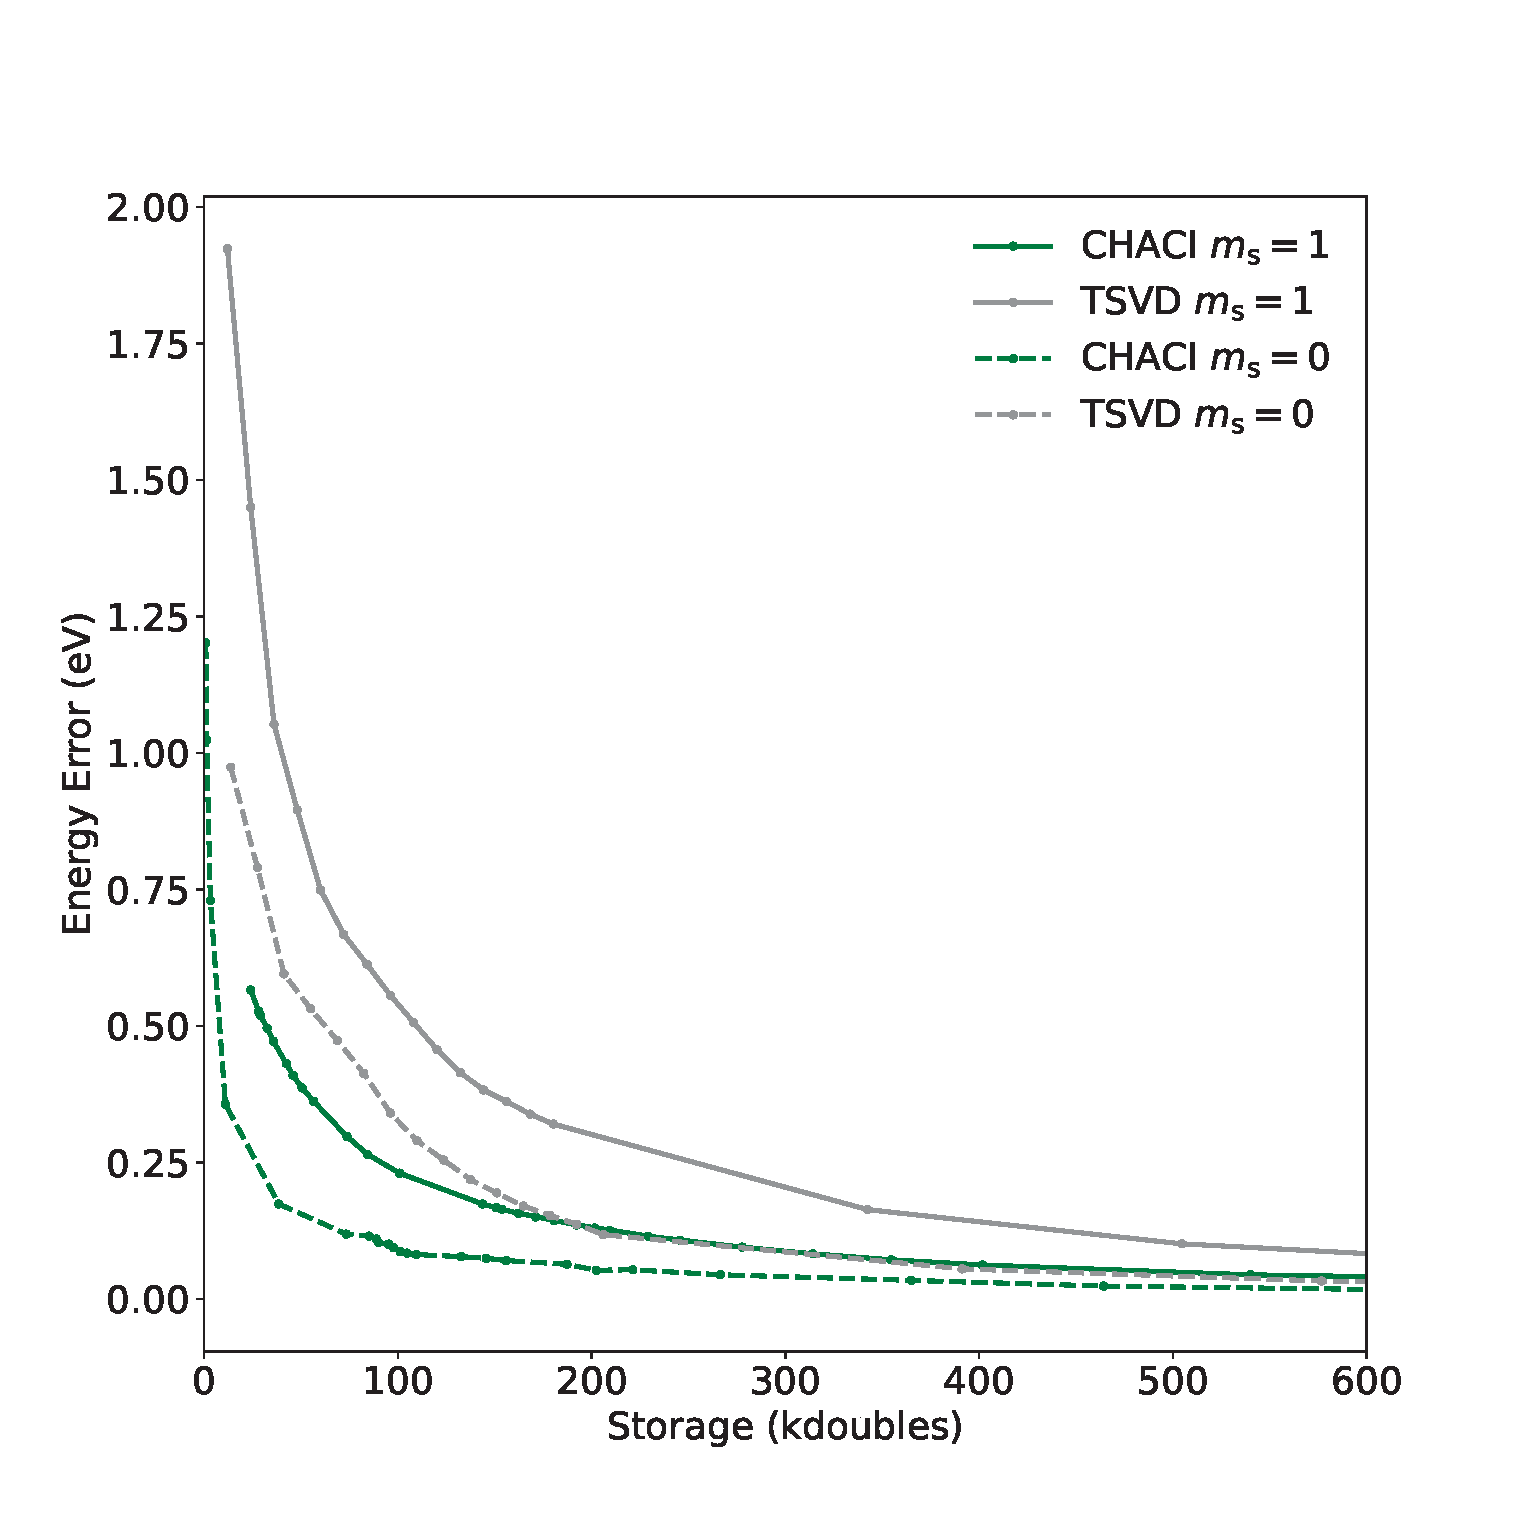
\includegraphics[width=0.5\linewidth]{figures/Degen_EN_Vs_St.eps}
    \caption{ The error in the absolute energies of two $m_s$ components of the triplet of 12-acene, computed with a 14-14 active space. Green and gray lines correspond to CHACI and TSVD, respectively.  Dashed and solid lines correspond to $m_s=0$ and $m_s=1$.}
    \label{fig:m_s_comparison-14-14}
\end{figure}

To investigate whether the convergence of states defined in different configuration spaces is balanced, we compare the convergence behavior of two rigorously degenerate states with very different CI vectors: the $m_s=0$ and $m_s=1$ components of the triplet (Fig. \ref{fig:m_s_comparison-14-14}).  The CHACI approach outperforms TSVD in all cases.  However, the $m_s=0$ wave function converges considerably more quickly with increasing storage than the $m_s=1$ wave function in both cases.  In addition, the discrepancy for CHACI is very large at some points, with the error in the absolute energy of the $m_s=1$ component being several times larger than that of the $m_s=0$ component.  This larger error is observed despite the fact that the $m_s=1$ CI vector is actually 24\% shorter than the $m_s=0$ vector.  It seems that achieving a balanced treatment of states defined in different configuration spaces is challenging.
}

\begin{figure}[htbp]
    \centering
    \includegraphics[width=0.6\linewidth]{figures/image6.eps}
    \caption{The error in the singlet-triplet gap of 12-acene as a function of total storage, computed with a 16-16 active space. The gray and green lines represent the error incurred by compression of the wave function using TSVD and CHACI, respectively.}
    \label{fig:error-gap-16-16}
\end{figure}

\begin{figure}[htbp]
    \centering
    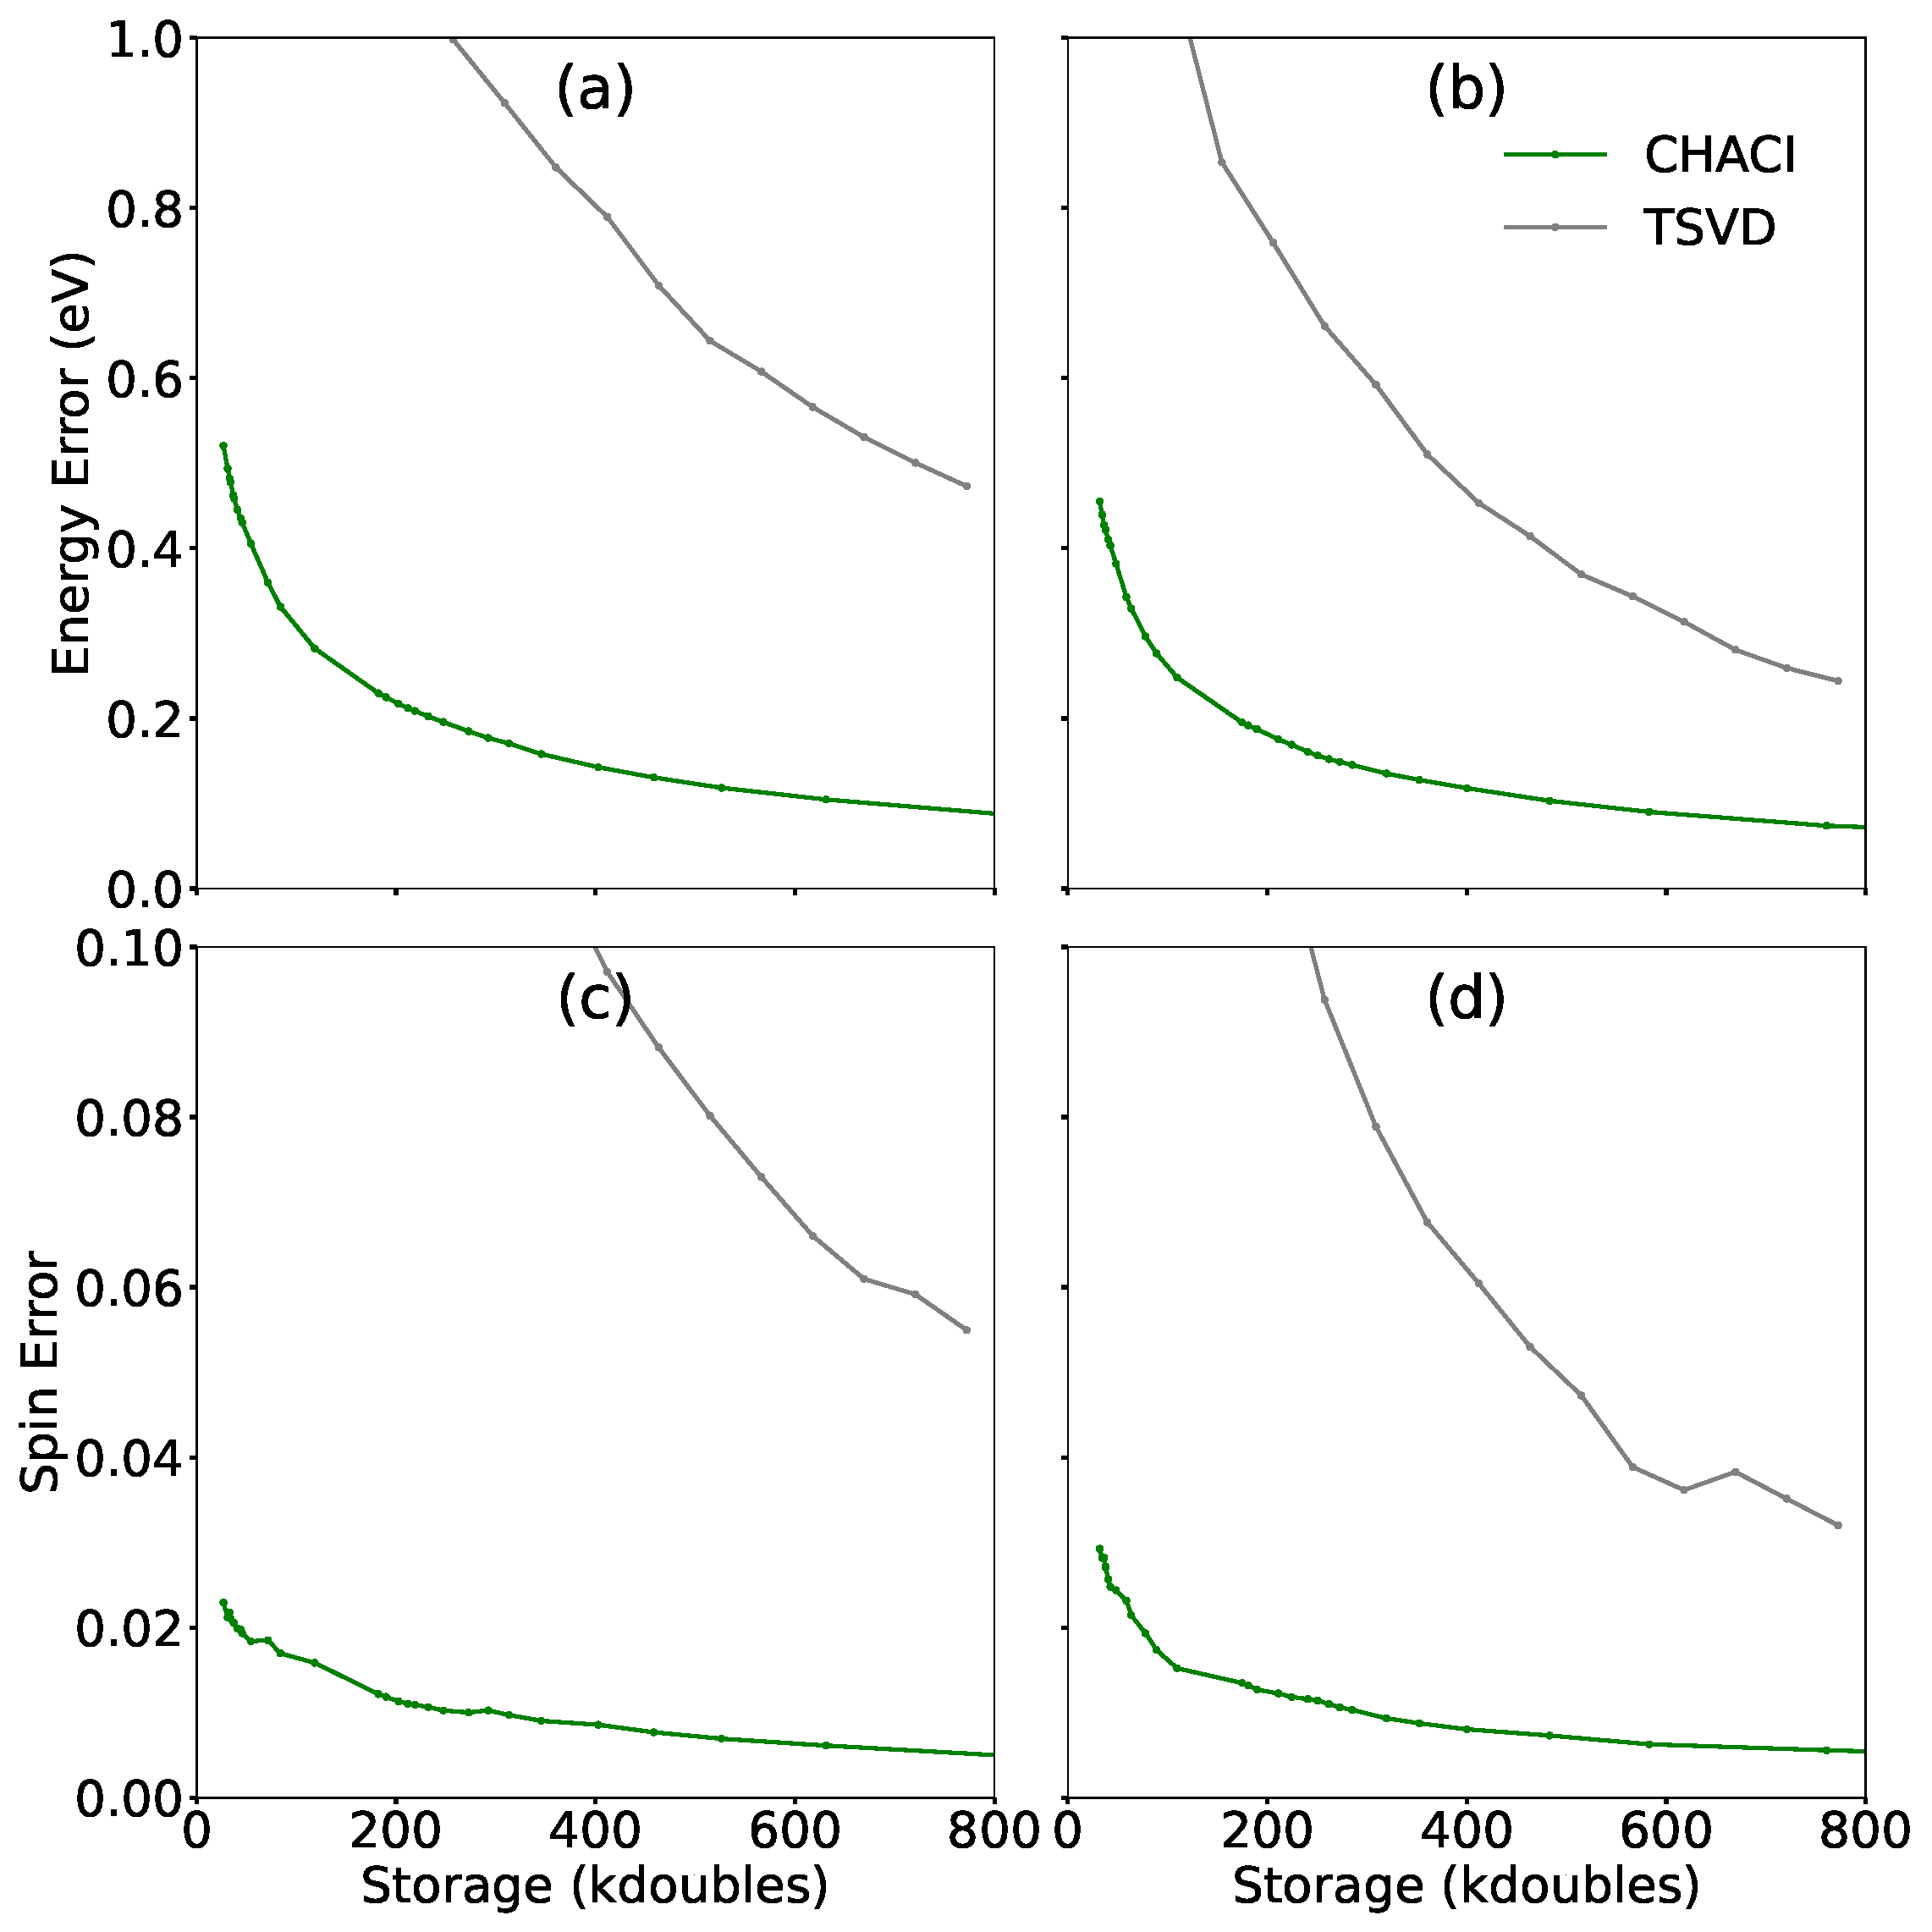
\includegraphics[width=6.50in, height=6.50in]{figures/image7.eps}
    \caption{Absolute energy (a and b) and spin (c and d) errors as a function of the storage for 12-acene with a 16-16 active space. Panel (a) and (c) correspond to the singlet wave function, while (b) and (d) correspond to the triplet wave function. The gray and green lines correspond to TSVD and CHACI compression, respectively.}
    \label{fig:energy-spin-errors-16-16}
\end{figure}

Figures~\ref{fig:error-gap-16-16} and \ref{fig:energy-spin-errors-16-16} demonstrate that the difference in performance between CHACI and TSVD increases when the active space size is increased from 14-14 to 16-16. In Figure~\ref{fig:error-gap-16-16}, it can be seen that errors in the singlet-triplet gap are at or below 0.1 eV for all cases, when CHACI is employed, even when only 59 kdoubles are stored (compared to 165,637 kdoubles for dense storage). Errors decrease rapidly with additional storage. In contrast, TSVD errors are above 0.2 eV for all cases. Similarly large differences in performance are observed for errors in absolute energy and spin in Figure~\ref{fig:energy-spin-errors-16-16}. As in the 14-14 case, CHACI does a much better job of maintaining the spin symmetry of the wave function than TSVD.

\subsection{Extrapolation of Performance to Larger Active Spaces}
\label{subsec:extrapolation-of-performance}
\begin{figure}[htbp]
    \centering
    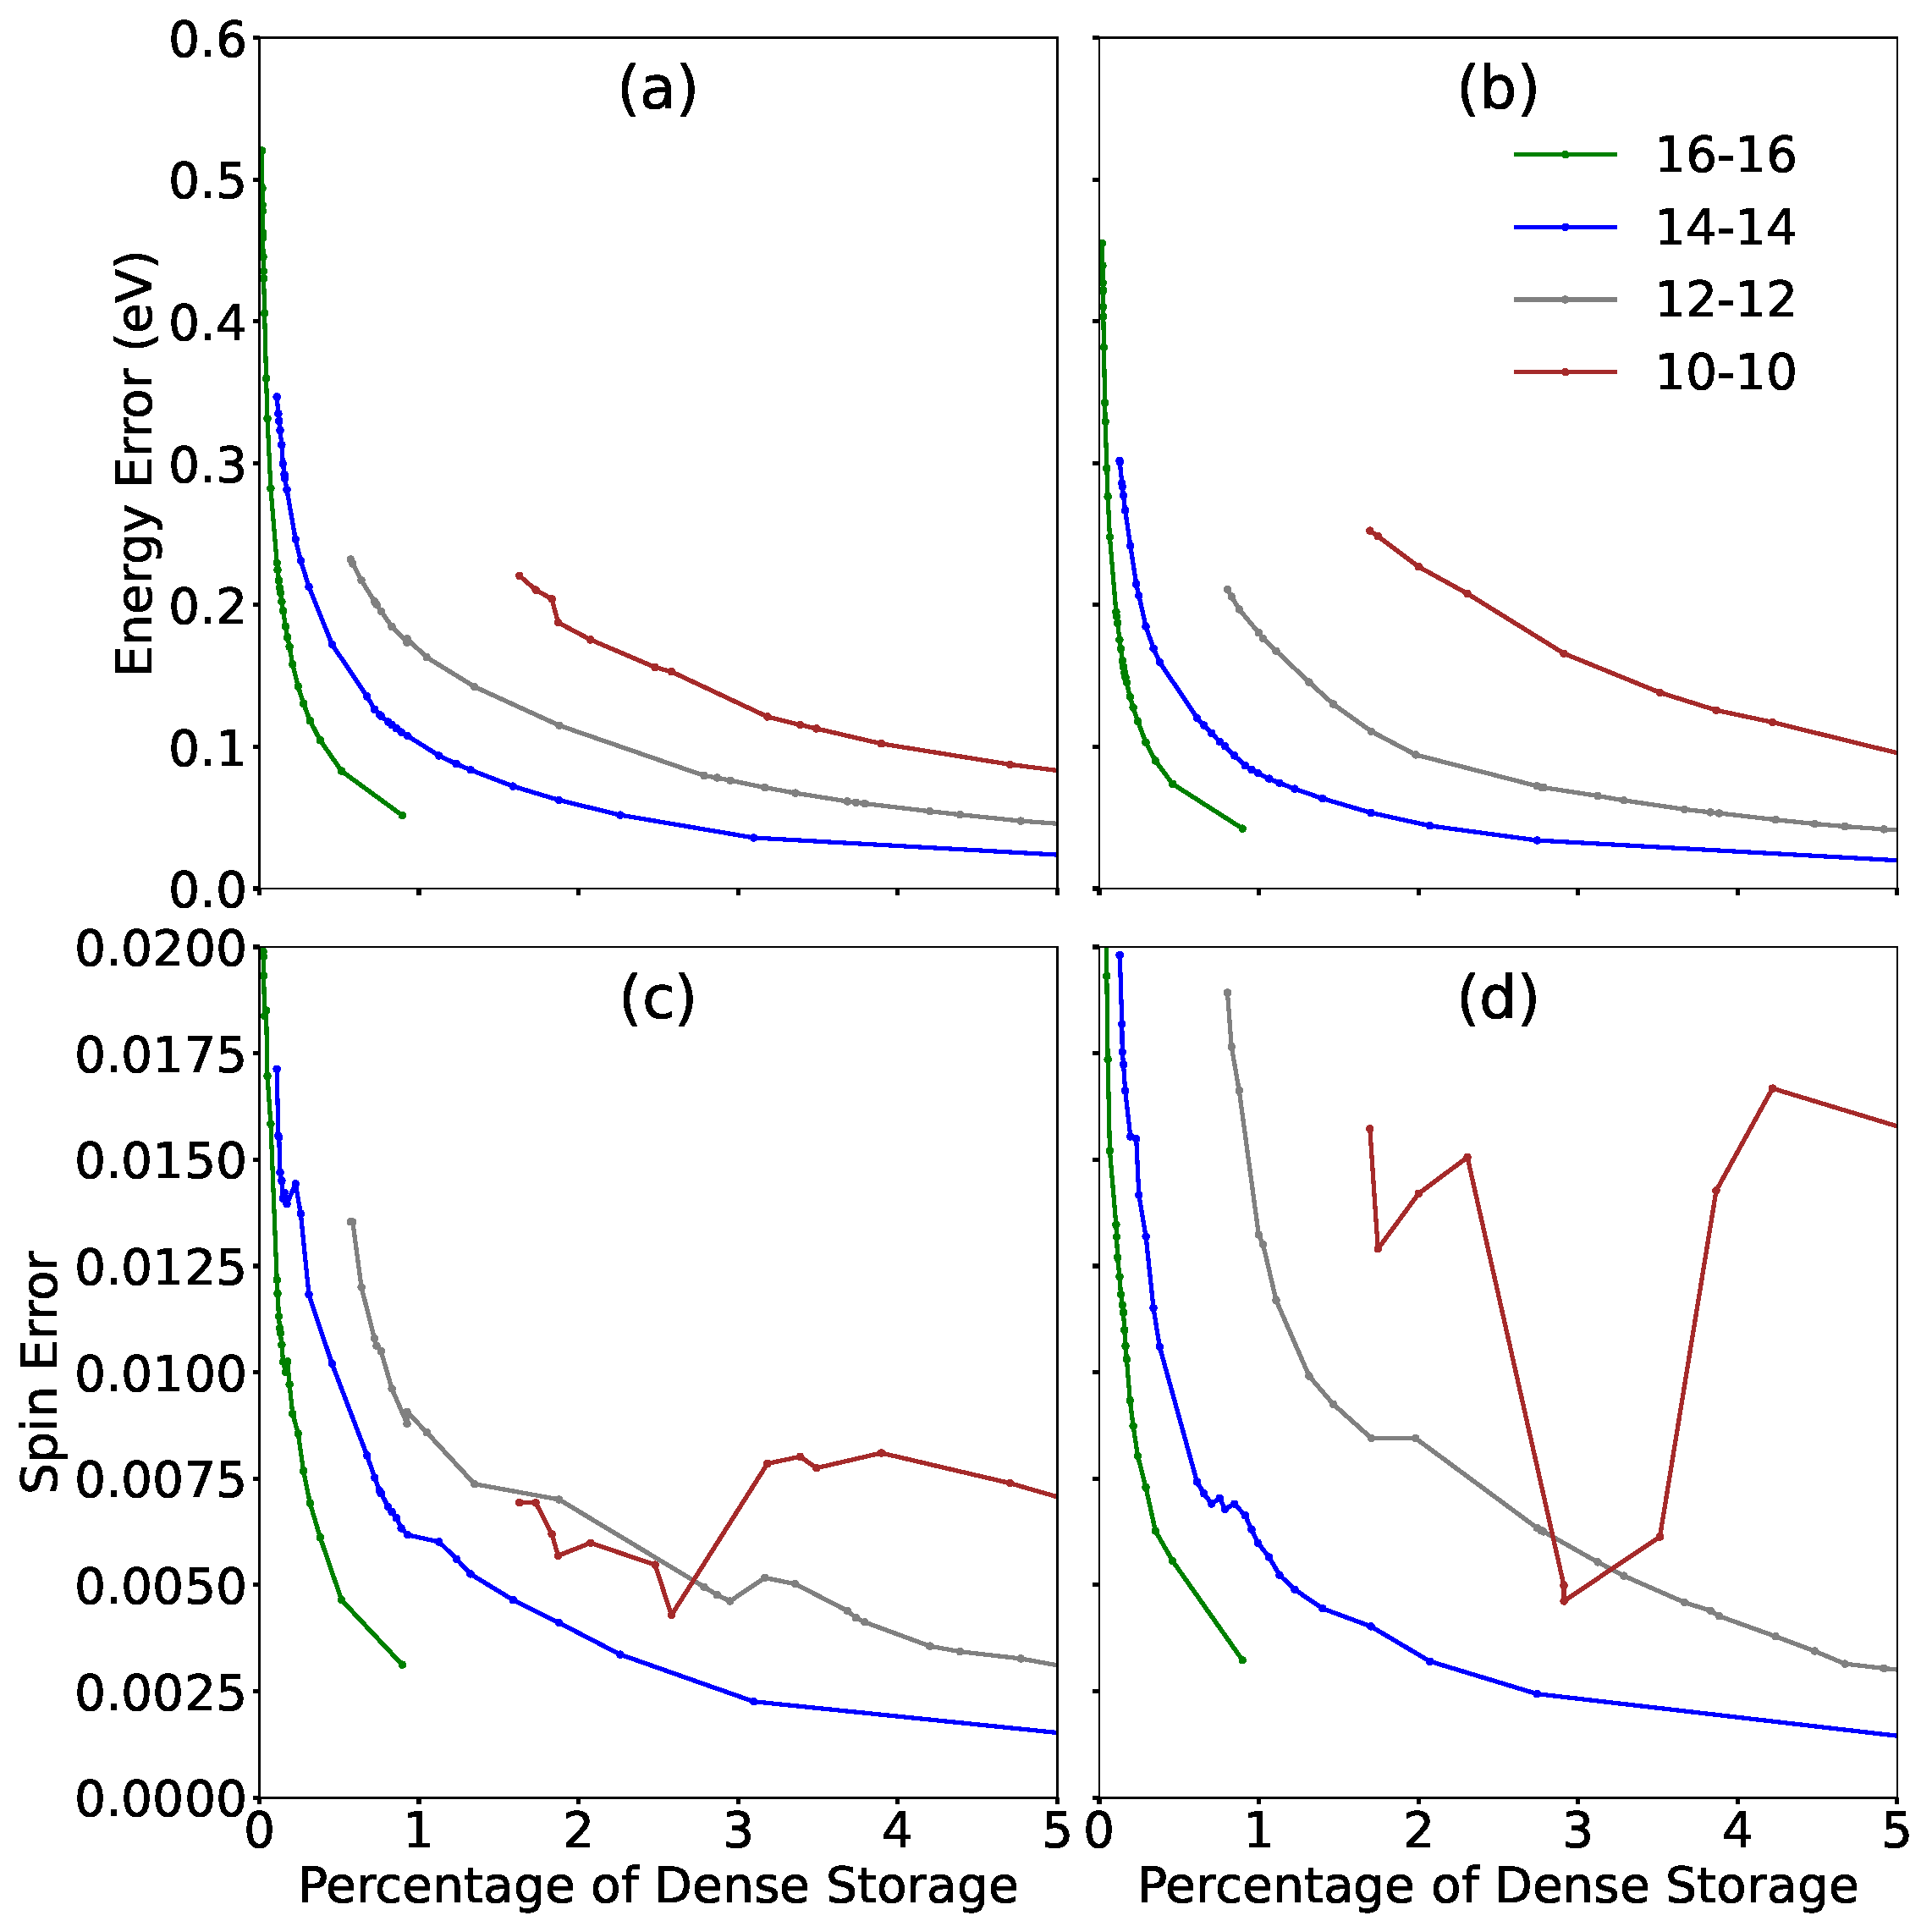
\includegraphics[width=5.89in, height=5.89in]{figures/image8.eps}
    \caption{The absolute energy (a and b) and spin errors (c and d) as a function of the percentage of dense storage for 12-acene with 10-10, 12-12, 14-14, and 16-16 active spaces. Panels (a) and (c) correspond to the singlet wave function, while panels (b) and (d) correspond to the triplet spin wave function.}
    \label{fig:errors-vs-compression-ratio}
\end{figure}

Ultimately, our goal is not to compute dense wave functions for subsequent compression. Our goal is to solve for large CI wave functions using a hierarchically compressed basis. Thus, in this section, we consider the behavior of CHACI compression as a function of active space size. In Figure~\ref{fig:errors-vs-compression-ratio}, we consider several active spaces, comparing the convergence of several measures of the accuracy as a function of the percentage of dense storage used (the compression ratio). We find that as the size of the active space increases, the accuracies of both absolute energy and spin converge faster with increasing compression ratio.

\begin{figure}[htbp]
    \centering
    \includegraphics[width=4.55in, height=4.45in]{figures/image9.eps}
    \caption{The storage ratio required to achieve \(<0.2\) eV accuracy in absolute energies as a function of the active space size. Blue and black lines correspond to the singlet and triplet wave functions, respectively.}
    \label{fig:compression-ratio-extrapolation}
\end{figure}

To quantify this convergence behavior, we plot the compression ratio at which absolute energies of 0.2 eV accuracy are achieved as a function of the number of active orbitals/electrons in Figure~\ref{fig:compression-ratio-extrapolation}. Both the singlet and triplet compression ratios converge quickly with increasing active space. Of the two, the triplet energy converges more slowly, thus we fit it to an exponential in order to extrapolate to larger active spaces. We find that the required compression ratio decays proportional to
\begin{equation}
f(N_\text{MO}) \propto e^{-0.561N_\text{MO}}.
\end{equation}
Extrapolating to larger active spaces, we estimate that a 24-24 active space could converge to 0.2 eV accuracy at a storage cost of 77,370 kdoubles, which is less than the cost of the dense storage of a 16-16 active space (165,637 kdoubles). Though the convergence behavior is likely to be system-dependent, this result certainly encourages further study.

{
\subsection{Effect of Compression on the Potential Energy Surface}
\label{subsec:effect-of-compression-on-the-pes}
\begin{figure}[htbp]
    \centering
    \includegraphics[height=4.0in]{figures/Singlet_PES.pdf}
    \caption{The PES of 12-acene as a function of the displacement of a single carbon atom out of plane, computed with a 14-14 active space.  Results in the low, medium, and high storage regimes ($\sim$50, $\sim$130, $\sim$190 kdoubles) are compared to exact CASCI results.}
    \label{fig:pes}
\end{figure}

It is interesting to consider how a potential energy surface (PES) is effected by compression for two reasons.  First, one might expect that compression might introduce non-parallelity error.  Second, as one moves from point to point along the PES, one might expect discontinuities as specific singular vector pairs are added or dropped.  

To investigate this possibility, we have computed the PES as a function of the out-of-plane displacement of a single carbon atom in 12-acene in three different storage regimes (Fig. \ref{fig:pes}).  No discontinuities are observed on the scale of 0.01 eV in any of the plots.  Comparing the energies at the first and last points of each curve, we observe very small deviations from parallelity: $5\times10^{-4}$, $3\times10^{-4}$, and $4\times10^{-5}$ eV in the low, medium, and high storage regimes, respectively.
}

\subsection{Effect of Using Optimal Rank on Compression}
\label{subsec:effect-of-dynamic-rank-on-compression}
\begin{figure}[htbp]
    \centering
    \includegraphics[width=6.41in, height=4.49in]{figures/image10.eps}
    \caption{The SR-CHACI error (blue) in the singlet-triplet gap of 12-acene as a function of total storage, computed with a 14-14 active space. The TSVD and CHACI errors (gray and green, respectively) are shown for comparison.}
    \label{fig:SR-CHACI-gap-error}
\end{figure}

In order to assess the necessity of the optimal rank procedure, we compare SR-CHACI (which uses a static rank) to CHACI and TSVD. Figure~\ref{fig:SR-CHACI-gap-error} presents the error in the singlet-triplet gap as a function of the total storage for the 14-14 active space. Excepting one fortunate point at 160 kdoubles, the accuracy of SR-CHACI is significantly worse than that of CHACI, but still better than TSVD. However, considering the error in the absolute energies of the singlet and triplet states separately (Figure 11a and b, respectively), it is clear that this is due to error cancellation. Errors in the absolute energy of the singlet state derived from the SR-CHACI wave function are similar to those of TSVD, and much greater than those of CHACI. Further, errors in the SR-CHACI triplet state are slightly larger than TSVD.

\begin{figure}[htbp]
    \centering
    \includegraphics[width=6.50in, height=6.50in]{figures/image11.eps}
    \caption{The SR-CHACI errors (blue) in the absolute energy (a and b) and spin (c and d) as a function of the storage for 12-acene (14-14 active space). Panels (a) and (c) correspond to the singlet wave function, while (b) and (d) correspond to the triplet wave function. The TSVD (gray) and CHACI (green) errors are shown for comparison.}
    \label{fig:SR-CHACI-energy-spin-errors}
\end{figure}

Analysis of spin errors tells a similar story. CHACI is much superior to SR-CHACI at reproducing the spin of the original wave function, and SR-CHACI has similar (and sometimes larger) spin errors compared to TSVD. Taken together, we conclude that optimal rank is an essential component of the CHACI algorithm.

\subsection{Effect of Sorting on Compression}
\label{subsec:effect-of-sorting-on-compression}
Here we assess the necessity of another feature of the CHACI compression algorithm: the sorting of rows/columns of the \(\mathbf{C}\) matrix prior to compression. To this end, we compare U-CHACI, in which the rows/columns remain unsorted, to CHACI and TSVD. Figure~\ref{fig:CI-vector-heatmap} presents a heat-map of the uncompressed \(\mathbf{C}\) matrix of the singlet (panels a and c) and triplet (b and d) wave functions before (a and b) and after (c and d) sorting. Note that sorting concentrates larger elements into the upper-left corner of the matrix.

\begin{figure}[htbp]
    \centering
    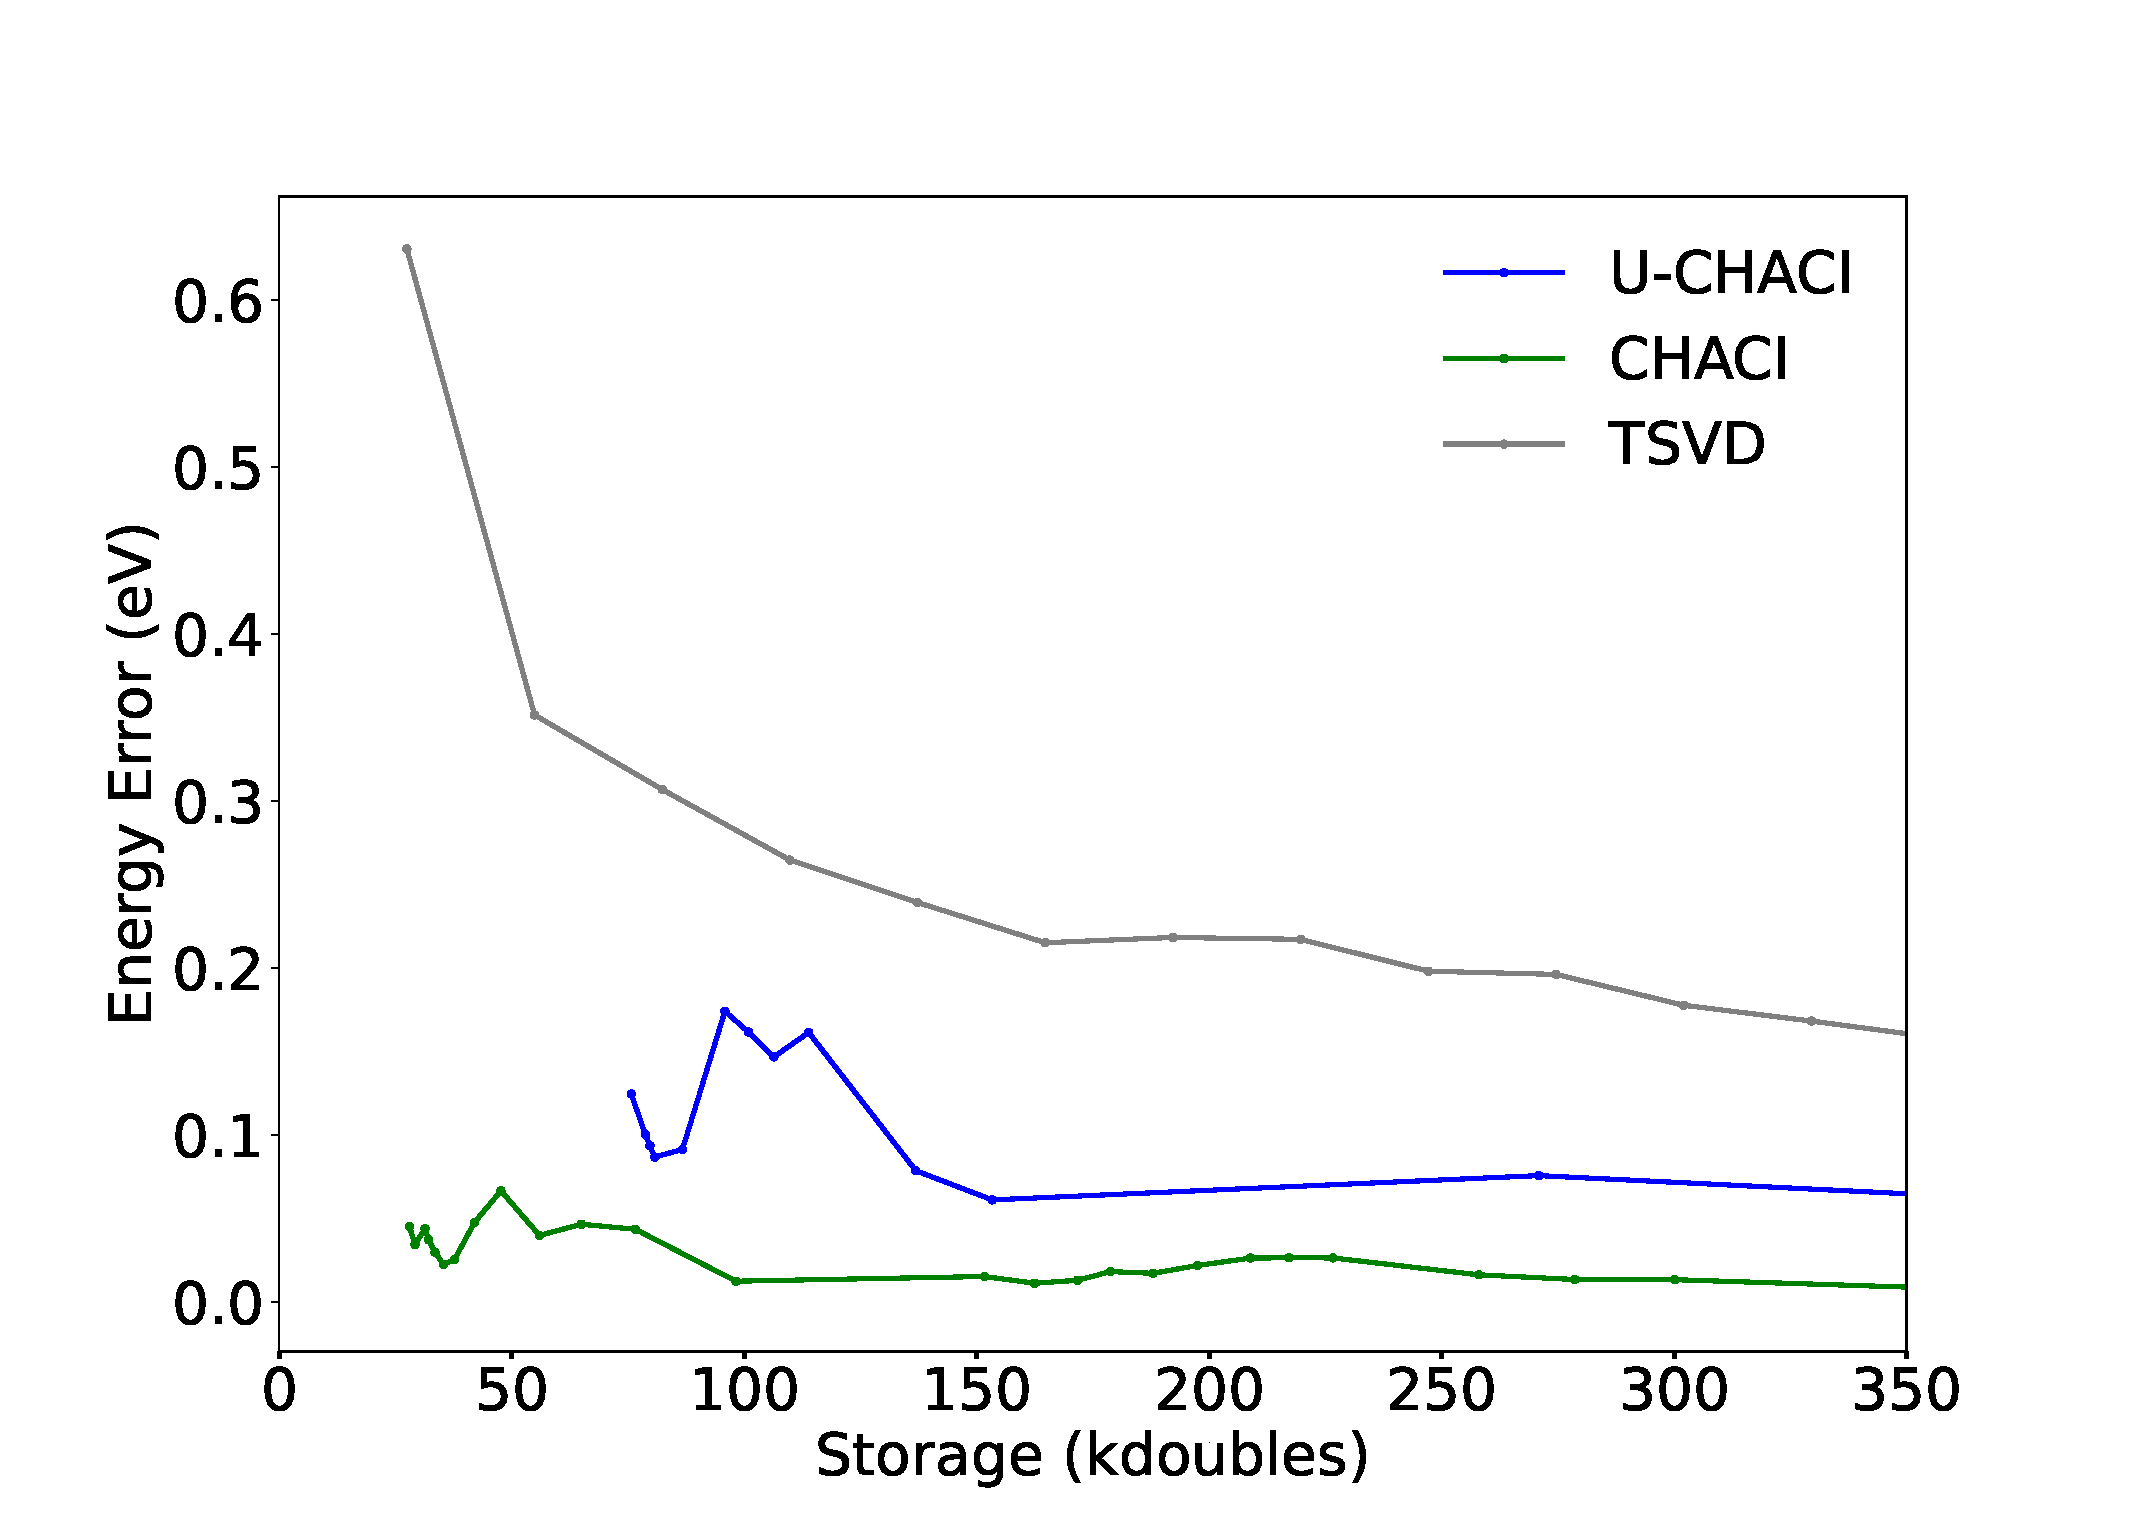
\includegraphics[width=4.59in, height=3.22in]{figures/image13.eps}
    \caption{The U-CHACI error (blue) in the singlet-triplet gap of 12-acene as a function of total storage, computed with a 14-14 active space. The TSVD and CHACI errors (gray and green, respectively) are shown for comparison.}
    \label{fig:U-CHACI-gap-error}
\end{figure}

Figure~\ref{fig:U-CHACI-gap-error} compares the U-CHACI singlet-triplet errors to those of CHACI and TSVD. Though U-CHACI appears to be more accurate for predicting the relative energy than TSVD, it remains inferior to CHACI. Considering the errors in the absolute singlet and triplet energies (Figure~\ref{fig:SR-CHACI-energy-spin-errors}a and b), we see that U-CHACI errors are on the order of the same size as those of TSVD, and considerably larger than those of CHACI. That being said, U-CHACI is solidly between CHACI and TSVD in its ability to accurately describe the total spin angular momentum (Figure~\ref{fig:SR-CHACI-energy-spin-errors}c and d).

\begin{figure}[htbp]
    \centering
    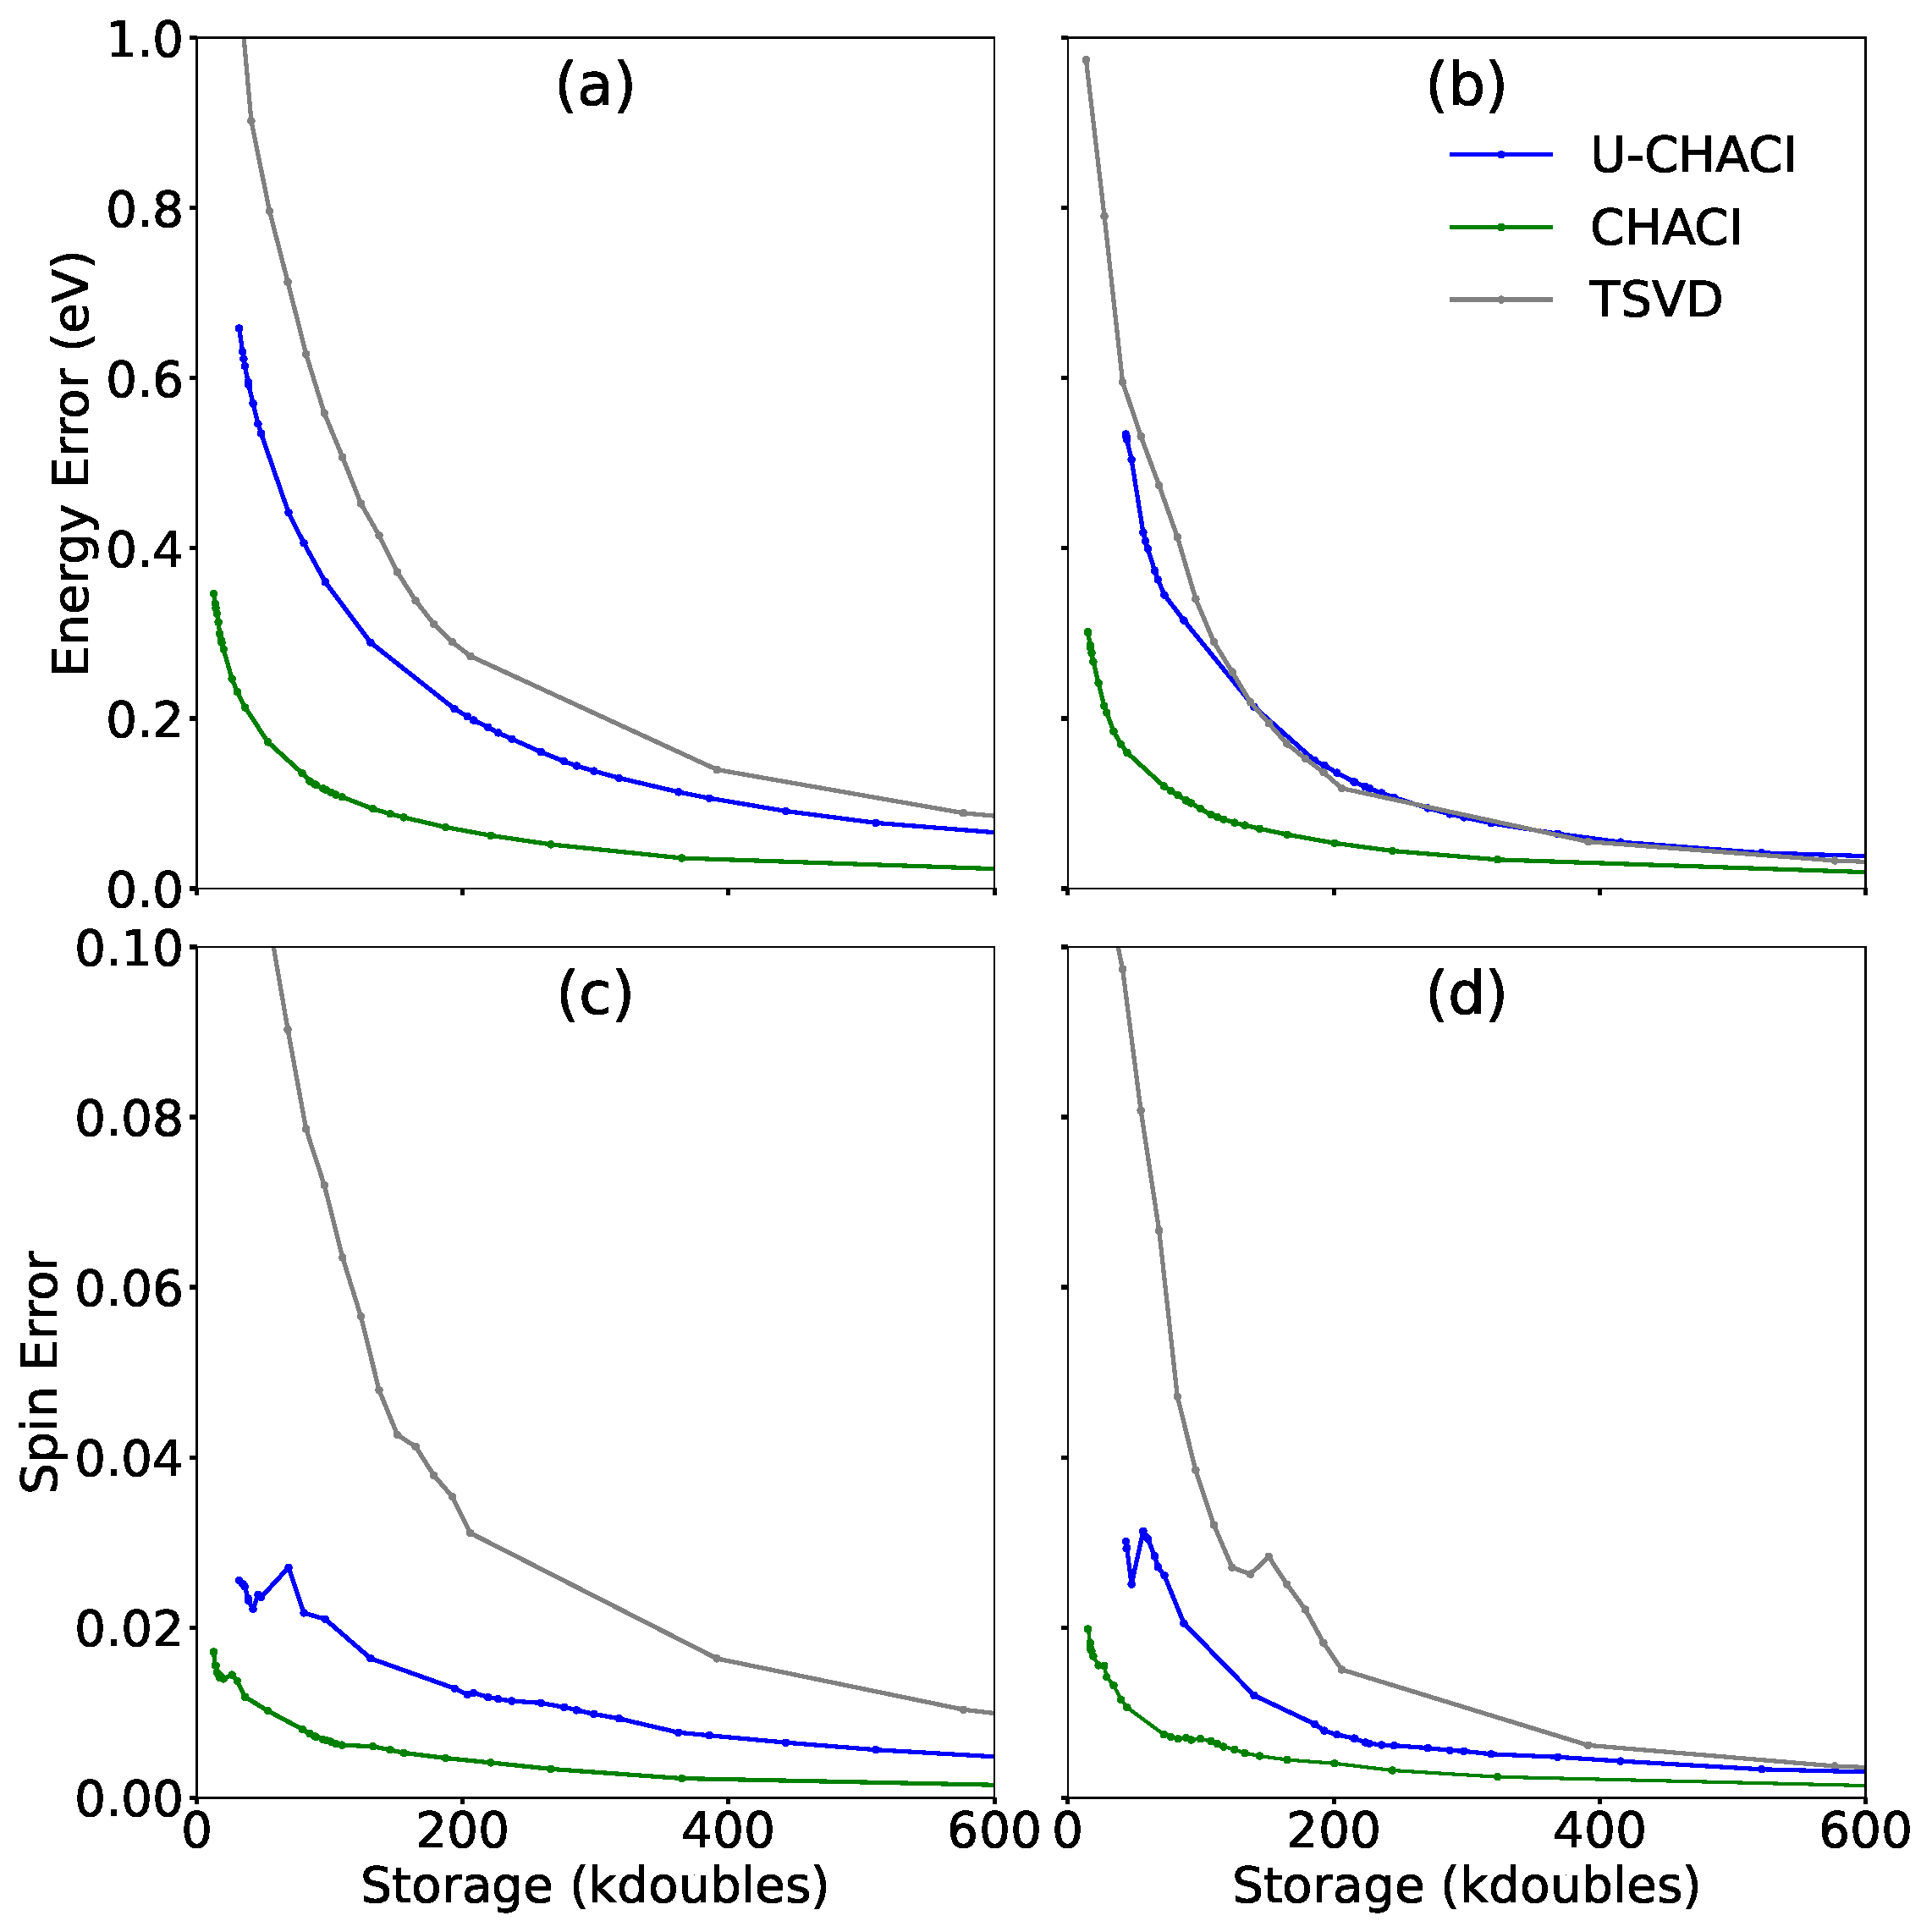
\includegraphics[width=4.26in, height=4.26in]{figures/image14.eps}
    \caption{The U-CHACI errors (blue) in the absolute energy (a and b) and spin (c and d) errors as a function of the storage for 12-acene (14-14 active space). Panels (a) and (c) correspond to the singlet wave function, while (b) and (d) correspond to the triplet wave function. The TSVD (gray) and CHACI (green) errors are shown for comparison.}
    \label{fig:U-CHACI-energy-spin-errors}
\end{figure}

Taking this data together, we conclude that sorting is an essential component of the CHACI algorithm. However, our ultimate goal is not to compute the full wave function and subsequently compress it, and the type of \textit{a posteriori} sorting that we use in CHACI would not be possible if we were to directly solve for the wave function in compressed form. But given that the Duch ordering of spin strings does not allow for efficient compression, the determination of an \textit{a priori} scheme by which strings may be ordered for efficient compression remains an important open question.

\subsection{Effect of Upper Quadrant vs H-matrix Compression}
\label{subsec:effect-of-upper-quadrant}
\begin{figure}[htbp]
    \centering
    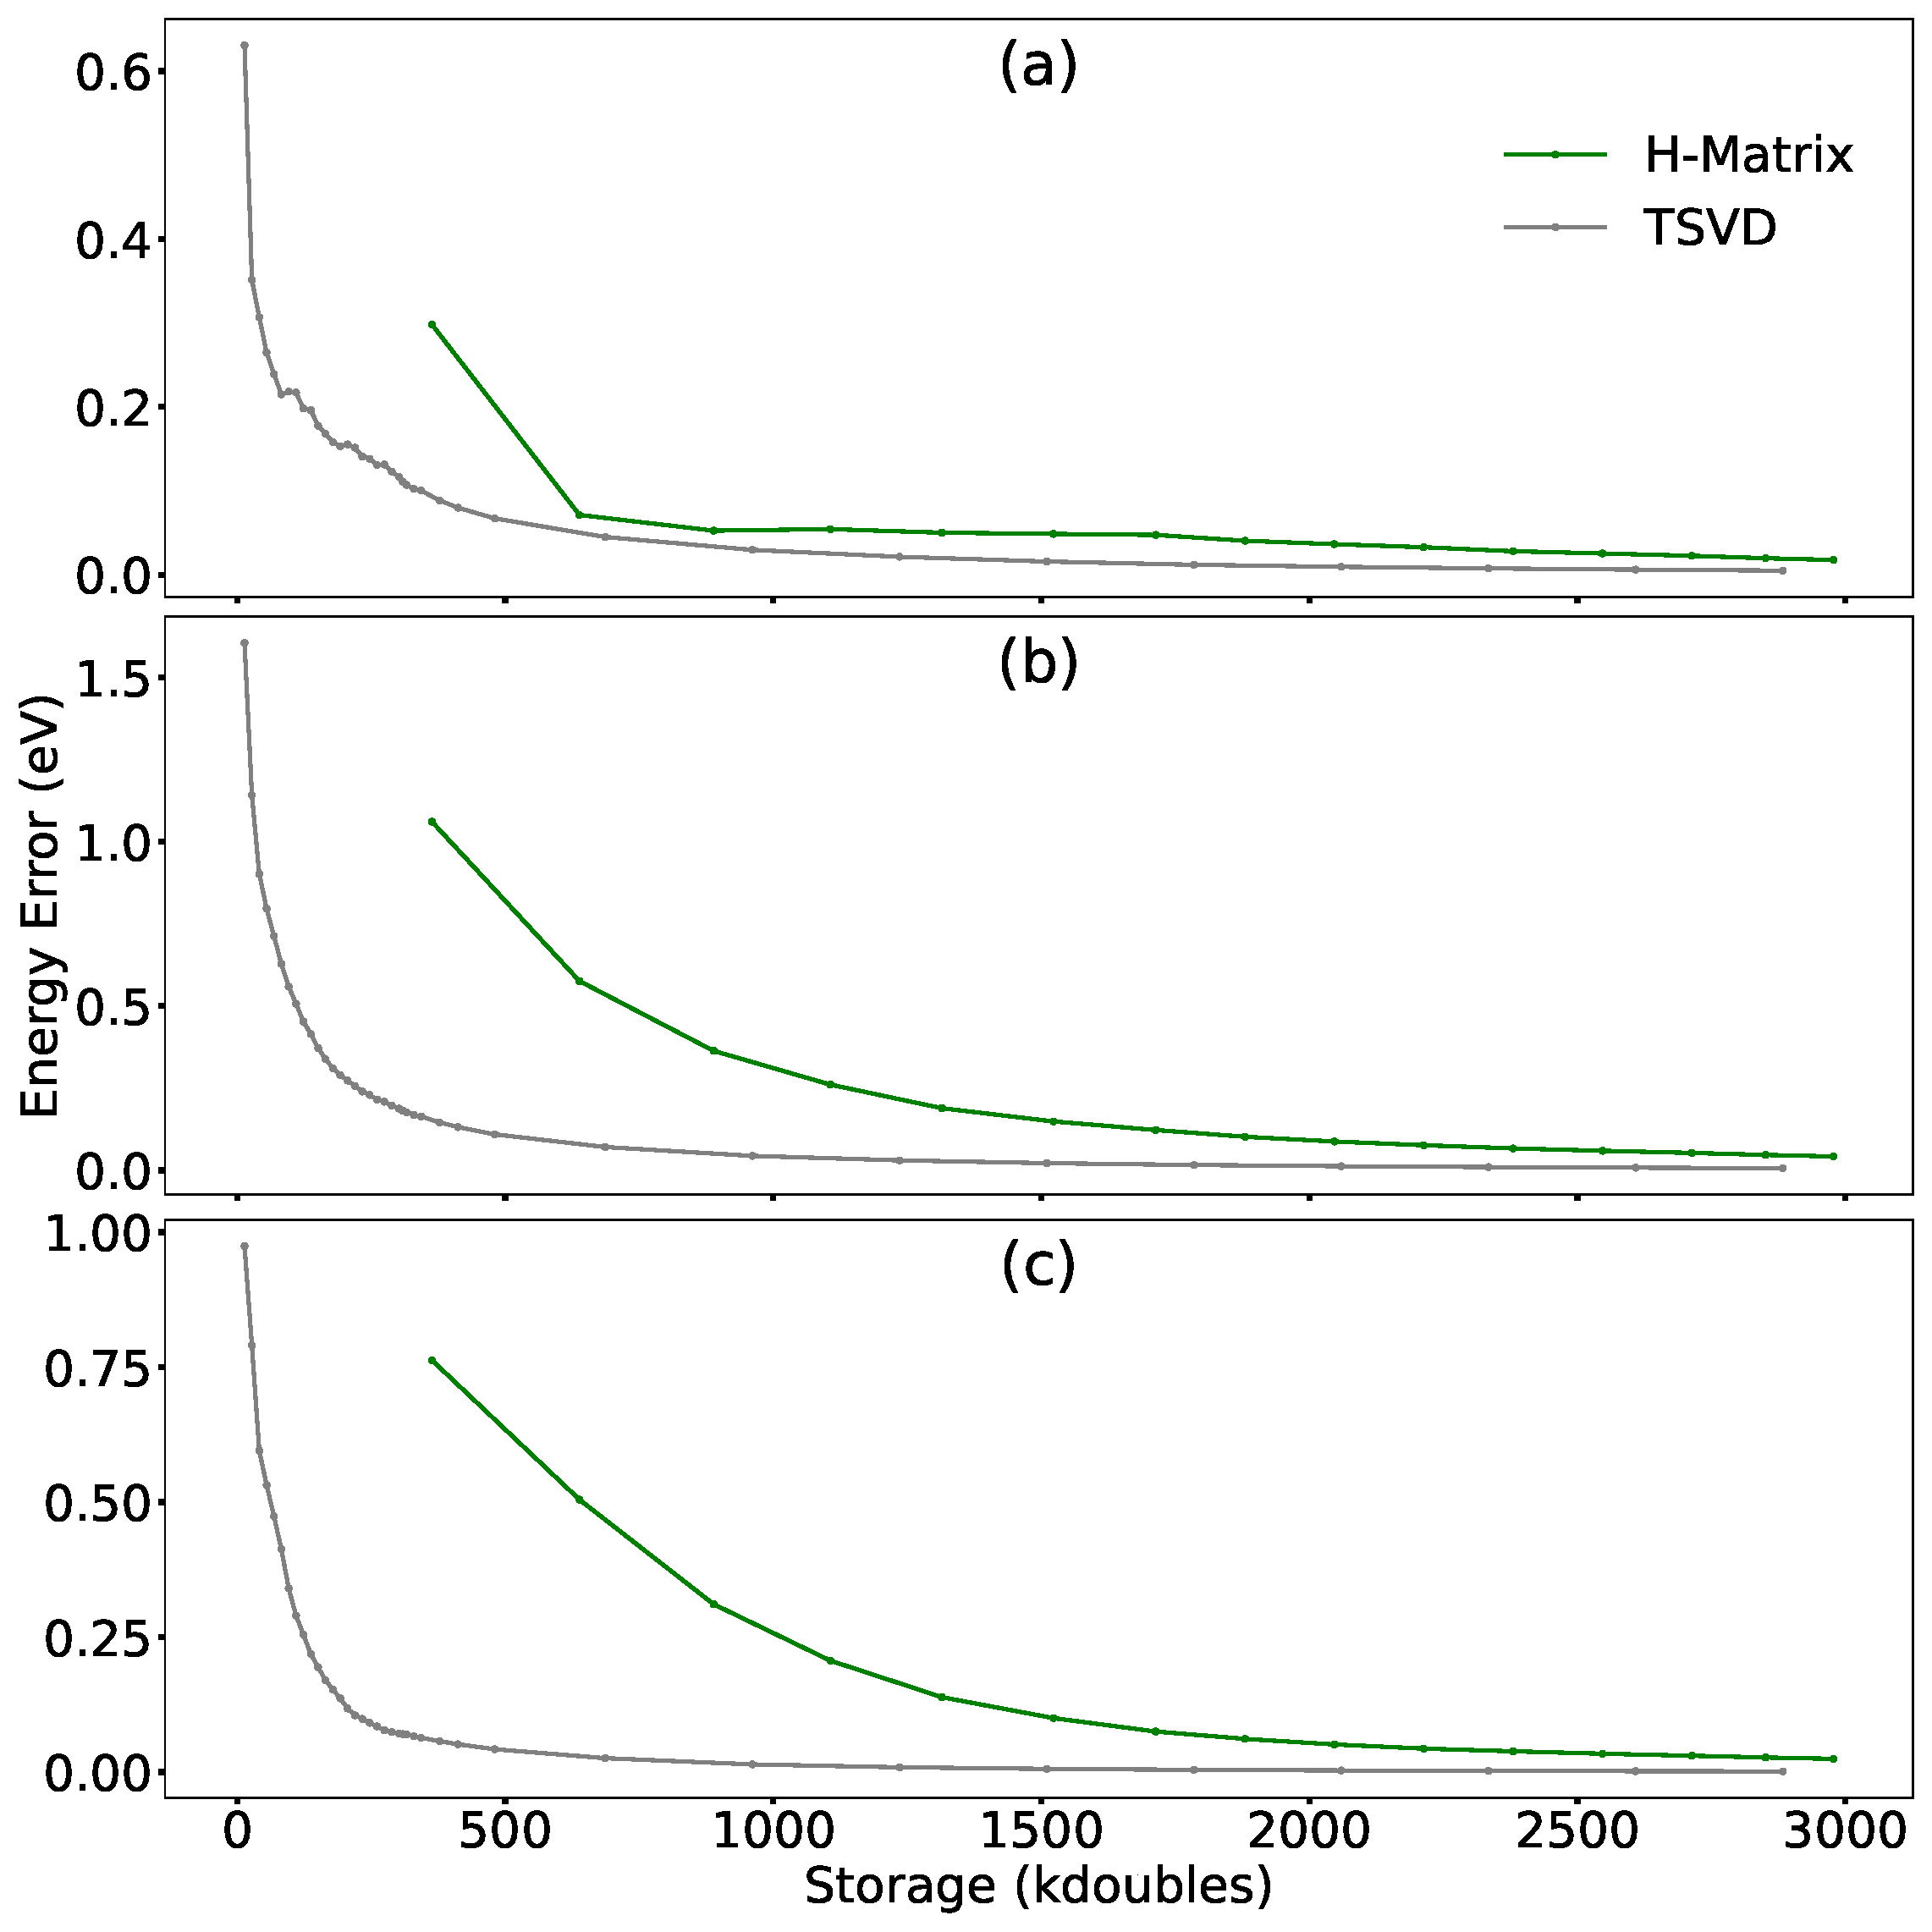
\includegraphics[width=4.79in, height=4.79in]{figures/H-Matrix.eps}
    \caption{Panels (a), (b), and (c) show the errors in the singlet-triplet gap, singlet, and triplet energies, respectively, of 12-acene (14-14 active space) as a function of the required storage for H-matrix and TSVD compression (green and gray).}
    \label{fig:H-matrix-vs-SVD}
\end{figure}

Lastly, we consider compression of \(\mathbf{C}\) into the H-matrix format,\cite{Hackbusch1999} which is designed to leverage the diagonally dominant nature of the matrix, in contrast to the CH blocking scheme used in CHACI. Figure~\ref{fig:H-matrix-vs-SVD} shows the error in the singlet-triplet gap, singlet absolute energy, and triplet absolute energy of the 14-14 wave function compressed into H-matrix format. H-matrix compression is inferior to TSVD, thus we conclude that the CH blocking scheme is an essential component of the CHACI scheme.